% This is part of Un soupçon de mathématique sans être agressif pour autant
% Copyright (c) 2014-2015
%   Laurent Claessens
% See the file fdl-1.3.txt for copying conditions.

%+++++++++++++++++++++++++++++++++++++++++++++++++++++++++++++++++++++++++++++++++++++++++++++++++++++++++++++++++++++++++++ 
\section{Non trié}
%+++++++++++++++++++++++++++++++++++++++++++++++++++++++++++++++++++++++++++++++++++++++++++++++++++++++++++++++++++++++++++

\begin{MentalActivity}
    \begin{mental}
        Calculer :
        \begin{enumerate}
            \item
                \( 18-12+3\)
            \item
                \( 3\times 8+2\)
            \item
                \( 3\times (8+2)\)
        \end{enumerate}
    \end{mental}

    \begin{mental}
        Vrai ou faux ?
        \begin{enumerate}
            \item
                \( 3\times (8+57)=3\times 8+57\)
            \item
                \( 12\times (32+3)=12\times 32+12\times 3\)
        \end{enumerate}
    \end{mental}
    
    \begin{mental}

        \begin{center}
   \input{Fig_RYDooDLpToB.pstricks}
        \end{center}
        
        Le périmètre du rectangle est
        \begin{enumerate}
            \item
                \( 2\times 15+\ell\)
            \item
                \( 15\times \ell\)
            \item
                \( 2\times (15+\ell)\)
        \end{enumerate}

    \end{mental}

    \begin{mental}
        \begin{enumerate}
            \item
                $\SI{250}{\centi\meter}=\ldots\si{\meter}$
            \item
                $\SI{1}{\liter}=\ldots\si{\deci\cubic\meter}$
            \item
                \( \SI{1}{\hour}=\ldots\si{\second}\)
        \end{enumerate}
    \end{mental}

\end{MentalActivity}

%%%%%%%%%%%%%%%%%%%%%%%%%%%%%%%%%%%%%%%%%%%%%%%%%%%%%%%%%%%%
\begin{MentalActivity}

    \begin{mental}
        Dire si les mesures suivantes sont les mesures d'un triangle (préciser si il est plat).
        \begin{enumerate}
            \item
                \( AB=5\), \( BC=7\), \( AC=10\)
            \item
                \( KL=9\), \( KT=1\),  \( LT=11\)
        \end{enumerate}
    \end{mental}

    \begin{mental}
        Quelle est la circonférence d'une cercle de rayon \( \SI{2}{\centi\meter}\) ? (rappel : la formule est \( 2\times\pi\times R\)) ?
    \end{mental}

    \begin{mental}
        Compléter :
        \begin{enumerate}
            \item
                \( 3\times 7-\ldots=15\)
            \item
                \( \dfrac{ 5\times 5\times 67 }{ 25 }=\ldots\)
            \item
                \( (100-5)\times 8=\ldots\times 100-\ldots\times 5\)
            \item
                \( \dfrac{ \ldots }{ 4+6 }=100\)
        \end{enumerate}
    \end{mental}

    \begin{mental}
        Trouver deux façons de compléter les mesures pour que les points \( A\), \( B\) et \( C\) soient alignés :
        \begin{subequations}
            \begin{align}
                AB&=\SI{5}{\centi\meter}\\
                BC&=\ldots\si{\centi\meter}\\
                AC&=\SI{4}{\centi\meter}
            \end{align}
        \end{subequations}
    \end{mental}
\end{MentalActivity}

\begin{MentalActivity}
    
    \begin{mental}
        Soit le programme de calcul
        \begin{framed}
            \begin{itemize}
                \item Choisir un nombre;
                \item soustraire \( 32\);
                \item diviser par 3
            \end{itemize}
        \end{framed}
        \begin{enumerate}
            \item
                De combien faut-il partir pour obtenir \( 6\) ?
            \item
                Combien obtient-t-on en partant de \( 101\) ?
        \end{enumerate}
    \end{mental}

    \begin{mental}
        Compléter les pointillés :
        \begin{enumerate}
            \item
                \( 5\times \ldots +5=30\)
            \item
                \( \dfrac{ 12\times 124 }{ \ldots }=124\)
            \item
                Le triangle de côtés \( AB=12\), \( BC=1\), \( AC=\ldots\) est isocèle.
        \end{enumerate}
    \end{mental}

    \begin{mental}
        Calculs 
        \begin{enumerate}
            \item
                Combien vaut \( 7\times a\) si \( a=9\) ?
            \item
                Combien vaut \( 2\times b+5\) si \( b=3\) ?
            \item
                Combien vaut \( 7\times a+b\) si \( a=2\) et \( b=6\) ?
        \end{enumerate}
    \end{mental}
\end{MentalActivity}

\begin{MentalActivity}
    \begin{mental}
        Quelle fraction va avec quel dessin ?
        \begin{multicols}{2}
            \begin{enumerate}
                \item
                    \( \dfrac{ 5 }{ 4 }\)
                \item
                    \( \dfrac{ 2 }{ 5 }\)
                \item
                    \( \dfrac{ 2 }{ 3 }\)
            \end{enumerate}

            \columnbreak

            \begin{enumerate}
   \item
   \input{Fig_RBEooLYHhMXooZERO.pstricks}
                \item
   \input{Fig_GVGooXlzMMh.pstricks}
   \item
   \input{Fig_RBEooLYHhMXooONE.pstricks}\( +\)\input{Fig_RBEooLYHhMXooTWO.pstricks}
            \end{enumerate}

        \end{multicols}
    \end{mental}

    \begin{mental}
        Écrire la réciproque des énoncés
        \begin{enumerate}
            \item
                Si un triangle a deux angles égaux, alors il est isocèle.
            \item
            Un nombre pair se termine par \( 0\), \( 2\), \( 4\), \( 6\) ou \( 8\).
        \end{enumerate}
    \end{mental}

    \begin{mental}
        \begin{enumerate}
            \item
                Combien vaut \( 3\times a+7\) si \( a=3\) ?
            \item
                Pour quelle valeur de \( a\) est-ce que \( 4\times a=16\) ?
            \item
                Pour quelle valeur de \( x\) est-ce que \( 2\times x+3=13\) ?
        \end{enumerate}
    \end{mental}
    
\end{MentalActivity}

\begin{MentalActivity}
% Ceci est dans mentaltruc 0057
% This is part of Un soupçon de mathématique sans être agressif pour autant
% Copyright (c) 2015
%   Laurent Claessens
% See the file fdl-1.3.txt for copying conditions.

    
    \begin{mental}
                L'aire de ce rectangle est de \(\SI{20}{\centi\meter\squared}\).
        \begin{center}
           \input{Fig_LCUooNGZJFk.pstricks}
        \end{center}
        Que vaut sa hauteur \( h\) ?
    \end{mental}


    \begin{mental}
        Calculer :
        \begin{enumerate}
            \item
                \( 103\times 12\)
            \item
                \( 7\times 0.81+0.19\times 7\).
        \end{enumerate}
    \end{mental}
    \begin{mental}
        L'aire du triangle \( ABC\) est \SI{30}{\centi\meter\squared}.

        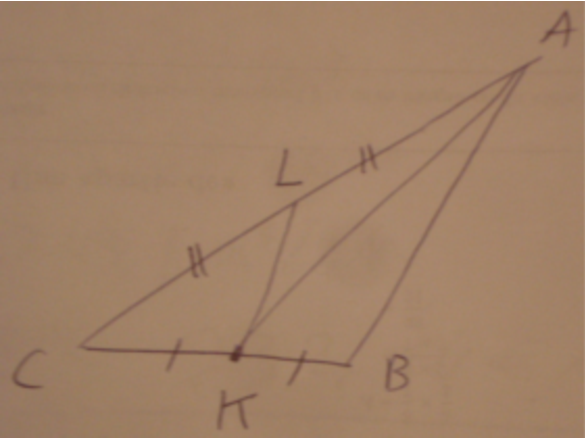
\includegraphics[width=10cm]{DSC01734.pdf}

        Quelle est l'aire de \( CKL\) ?
    \end{mental}
\end{MentalActivity}

\begin{MentalActivity}
    \begin{mental}
        Calculer :
        \begin{enumerate}
            \item
                \( \dfrac{ 1 }{ 2 }+\dfrac{ 1 }{ 4 }\)
            \item
                \( \dfrac{ 5 }{ 6 }-\dfrac{ 1 }{ 12 }\).
        \end{enumerate}
    \end{mental}
    \begin{mental}
        Un gaulois meurt en l'an \( 13\) à l'âge de \( 35\) ans. Quelle est son année de naissance ?
    \end{mental}
    \begin{mental}
        Le segment \( [DE]\) mesure \SI{7}{\centi\meter}. Quelle est la longueur de \( [BK]\) ?
        \begin{center}
            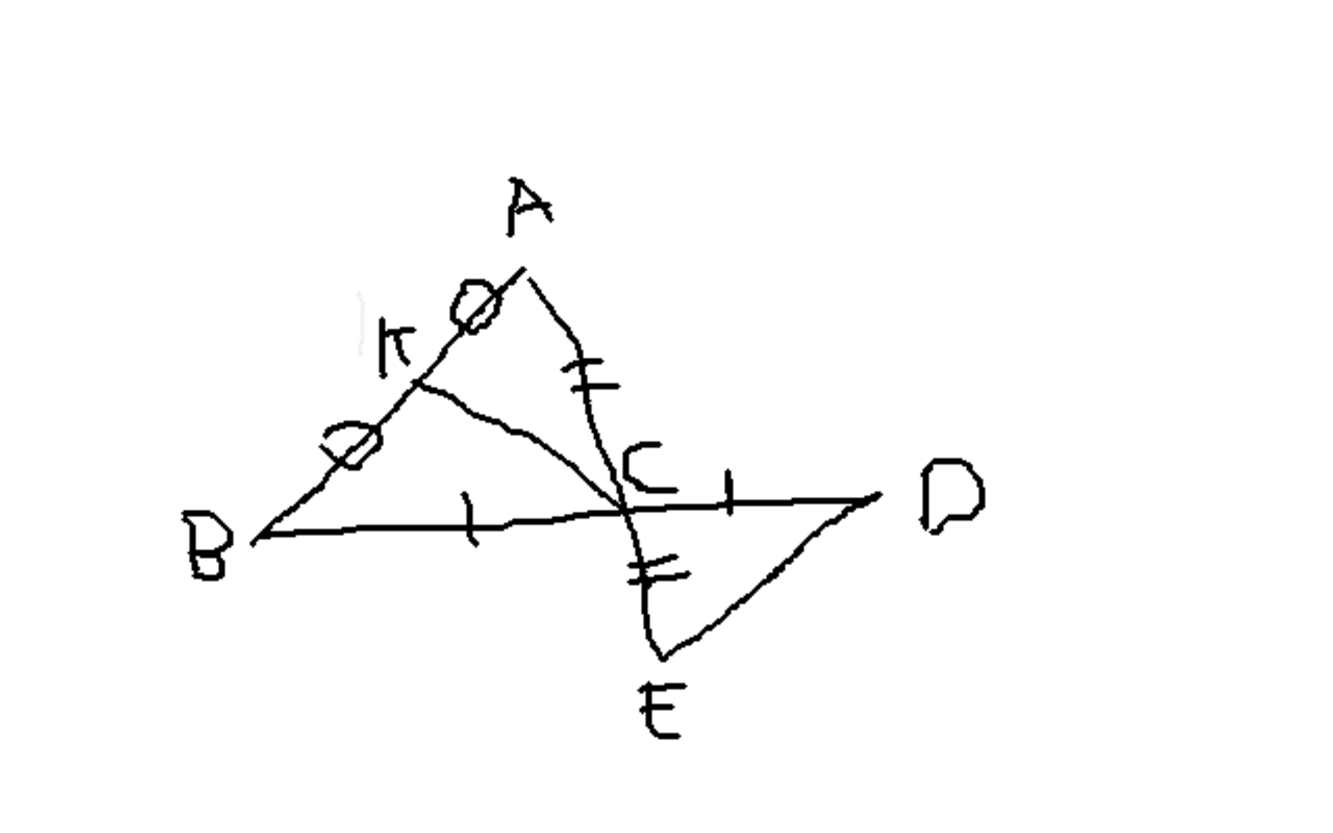
\includegraphics[width=20cm]{triangle_mental.pdf}
        \end{center}
    \end{mental}
\end{MentalActivity}

\begin{MentalActivity}
    \begin{mental}
        Calculer
        \begin{enumerate}
            \item
                \( \dfrac{ 5 }{ 7 }+\dfrac{ 2 }{ 7 }\)
            \item
                \( 1+\dfrac{ 5 }{ 7 }\)
        \end{enumerate}
    \end{mental}
    \begin{mental}
        Compléter les pointillés :
        \begin{enumerate}
            \item
                \( -3> \ldots\)
            \item
                \( \dfrac{ 4 }{ 10 }+\dfrac{ \ldots }{ 10 }=\dfrac{ 1 }{2}\)
        \end{enumerate}
    \end{mental}
    \begin{mental}
        Quelle est l'abscisse du symétrique du point \( A\) par rapport au point \( K\) ?
        \begin{center}
            \Large
            \input{Fig_GRBOooIZYhIV.pstricks}
        \end{center}
    \end{mental}
\end{MentalActivity}


% les deux cinquièmes ont fait celle-ci.
\begin{MentalActivity}          
% This is part of Un soupçon de mathématique sans être agressif pour autant
% Copyright (c) 2015
%   Laurent Claessens
% See the file fdl-1.3.txt for copying conditions.

    \begin{mental}
        Est-ce que les droites sont parallèles ?
\begin{center}
    \Large
\input{Fig_TVRGooTuCNyN.pstricks}
\end{center}
    \end{mental}

% This is part of Un soupçon de mathématique sans être agressif pour autant
% Copyright (c) 2015
%   Laurent Claessens
% See the file fdl-1.3.txt for copying conditions.

    \begin{mental}
        Lesquelles des deux maisons sont symétriques l'une de l'autre par rapport au point \( O\) ?
\begin{center}
    \large
   \input{Fig_NUEGooGTqxcl.pstricks}
\end{center}
    \end{mental}
         % Symétrie centrale
% This is part of Un soupçon de mathématique sans être agressif pour autant
% Copyright (c) 2015
%   Laurent Claessens
% See the file fdl-1.3.txt for copying conditions.

    \begin{mental}
        Si \( 6\) paquets de bonbons coûtent \( 3\) euros et \( 5\) paquets en coûtent \( 2.5\),
        \begin{enumerate}
            \item
                combien coûtent \( 10\) paquets de bonbons ?
            \item
                combien coûtent \( 11\) paquets de bonbons ?
        \end{enumerate}
    \end{mental}

% This is part of Un soupçon de mathématique sans être agressif pour autant
% Copyright (c) 2015
%   Laurent Claessens
% See the file fdl-1.3.txt for copying conditions.

    \begin{mental}
        Compléter avec l'entier le plus proche :
        \begin{enumerate}
            \item
                \( 5.3>\ldots\)
            \item
                \( -10<\ldots\)
            \item
                \( -5.3<\ldots\)
        \end{enumerate}
    \end{mental}
         % Compléter avec l'entier le plus proche
\end{MentalActivity}

%+++++++++++++++++++++++++++++++++++++++++++++++++++++++++++++++++++++++++++++++++++++++++++++++++++++++++++++++++++++++++++ 
\section{Mental 5A}
%+++++++++++++++++++++++++++++++++++++++++++++++++++++++++++++++++++++++++++++++++++++++++++++++++++++++++++++++++++++++++++
\setcounter{numactivmentale}{0}

% Pour 5A, 20 mars 2015
\begin{MentalActivity}  
% This is part of Un soupçon de mathématique sans être agressif pour autant
% Copyright (c) 2015
%   Laurent Claessens
% See the file fdl-1.3.txt for copying conditions.

\begin{mental}
    Développer :
            \begin{equation}
                5\times (12-x)
            \end{equation}
\end{mental}

% This is part of Un soupçon de mathématique sans être agressif pour autant
% Copyright (c) 2015
%   Laurent Claessens
% See the file fdl-1.3.txt for copying conditions.

   %tableau de proportionnalité
% This is part of Un soupçon de mathématique sans être agressif pour autant
% Copyright (c) 2015
%   Laurent Claessens
% See the file fdl-1.3.txt for copying conditions.


\begin{mental}
    
Sur ce dessin, \( (BD)\) est perpendiculaire à \( (BC)\).


\begin{center}
\input{Fig_HRIVooBXxZES.pstricks}
\end{center}

\end{mental}


\end{MentalActivity}

% Pour le 10 avril
\begin{MentalActivity}
% This is part of Un soupçon de mathématique sans être agressif pour autant
% Copyright (c) 2015
%   Laurent Claessens
% See the file fdl-1.3.txt for copying conditions.

\begin{mental}
    kmlkmlk
\end{mental}
<++>


% This is part of Un soupçon de mathématique sans être agressif pour autant
% Copyright (c) 2015
%   Laurent Claessens
% See the file fdl-1.3.txt for copying conditions.

\begin{mental}
    Calculer :
    \begin{enumerate}
        \item
            \( 7-5\)
        \item
            \( 5-7\)
        \item
            \( \frac{ 1 }{2}-1\)
    \end{enumerate}

    \vspace{2cm}

\begin{center}
   \input{Fig_FSQMooFDOrkR.pstricks}
\end{center}

\end{mental}

% This is part of Un soupçon de mathématique sans être agressif pour autant
% Copyright (c) 2015
%   Laurent Claessens
% See the file fdl-1.3.txt for copying conditions.


\begin{mental}

\begin{center}
    \large
   \input{Fig_KYVAooVmGYhS.pstricks}
\end{center}

    \( \hat K=\ldots\)
\end{mental}

\end{MentalActivity}

% Pour le 22 mai
\begin{MentalActivity}
% This is part of Un soupçon de mathématique sans être agressif pour autant
% Copyright (c) 2015
%   Laurent Claessens
% See the file fdl-1.3.txt for copying conditions.

\begin{mental}
    \begin{enumerate}
        \item
            Combien d'euros et de centimes dans \( 1.5\)€ ?
        \item
            Combien d'heures et de minutes dans \SI{1.5}{\hour} ?
        \item
            Combien de kilos et de grammes dans \SI{1.5}{\kilo\gram} ?
    \end{enumerate}
\end{mental}

% This is part of Un soupçon de mathématique sans être agressif pour autant
% Copyright (c) 2015
%   Laurent Claessens
% See the file fdl-1.3.txt for copying conditions.

\begin{mental}
    klmk
UFBQooOXIMjV


\begin{center}                                                                                                                                                                                                     \input{Fig_UFBQooOXIMjVooZERO.pstricks}                                                                                                                                                      
\end{center} 


\begin{center}
   \input{Fig_UFBQooOXIMjVooONE.pstricks}
\end{center}

\end{mental}
<++>

% This is part of Un soupçon de mathématique sans être agressif pour autant
% Copyright (c) 2015
%   Laurent Claessens
% See the file fdl-1.3.txt for copying conditions.

\begin{mental}
    Laquelle de ces deux égalités est correcte si \( x=-100\) ?

    \begin{enumerate}
        \item
    $100-x=0$
\item
    $x+100=0$
    \end{enumerate}
\end{mental}


\end{MentalActivity}

% Pour le 5 juin
\begin{MentalActivity}
% This is part of Un soupçon de mathématique sans être agressif pour autant
% Copyright (c) 2015
%   Laurent Claessens
% See the file fdl-1.3.txt for copying conditions.

\begin{mental}
    
Voici les éphémérides d'une éclipse\cite{PMUPooZAPegi}.
    \begin{center}
    \begin{tabular}[]{|c|c|}
        \hline
        Entrée dans l'ombre&6h58\\
        \hline
        Commencement de la totalité de l'éclipse&8h06\\
        \hline
        Maximum de l'éclipse&8h45\\
        \hline
        Fin de la totalité de l'éclipse&9h24\\
        \hline
        Sortie de l'ombre de la Terre&10h33\\
        \hline
    \end{tabular}
    \end{center}
    Pendant combien de temps l'éclipse est-elle totale ?

\end{mental}

% This is part of Un soupçon de mathématique sans être agressif pour autant
% Copyright (c) 2015
%   Laurent Claessens
% See the file fdl-1.3.txt for copying conditions.

\begin{mental}
    
    Quelle est la longueur totale des arrêtes ?

\begin{center}
    \input{Fig_GJMFooFKVCyK.pstricks}
\end{center}

\end{mental}

% This is part of Un soupçon de mathématique sans être agressif pour autant
% Copyright (c) 2015
%   Laurent Claessens
% See the file fdl-1.3.txt for copying conditions.

\begin{mental}
    

Aire \( DEF\) : \SI{5}{\meter\squared}.

\begin{center}
   \input{Fig_GOARooHSKUuw.pstricks}
\end{center}

Aire \( ABC\) ?


\end{mental}

\end{MentalActivity}

% Pour le 19 juin
\begin{MentalActivity}
% This is part of Un soupçon de mathématique sans être agressif pour autant
% Copyright (c) 2015
%   Laurent Claessens
% See the file fdl-1.3.txt for copying conditions.

\begin{mental}
    Compléter avec l'entier le plus proche possible :
    \begin{enumerate}
        \item
            \( -5<\ldots\)
        \item
            \( \ldots<8.2\)
        \item
            \( -1.9>\ldots\)
    \end{enumerate}
\end{mental}

% This is part of Un soupçon de mathématique sans être agressif pour autant
% Copyright (c) 2015
%   Laurent Claessens
% See the file fdl-1.3.txt for copying conditions.

\begin{mental}
Quel est l'intrus ?
\begin{multicols}{2}
\begin{enumerate}
    \item
        \( 25\%\)
    \item
        \( \dfrac{1}{ 25 }\)
    \item
        \( 0.25\)
    \item
        \( \dfrac{ 25 }{ 100 }\)
    \item
        \( \dfrac{ 50 }{ 200 }\)
\end{enumerate}
\end{multicols}
\end{mental}

% This is part of Un soupçon de mathématique sans être agressif pour autant
% Copyright (c) 2015
%   Laurent Claessens
% See the file fdl-1.3.txt for copying conditions.

\begin{mental}
    Répartition des animaux dans un zoo :
    \begin{center}
    \begin{tabular}[]{|c||c|}
        \hline
        proportion (en \%)&type\\
        \hline\hline
        \( 13\)&reptiles\\
        \hline
        \ldots&oiseaux\\
        \hline
        60&mammifères\\
        \hline
        9&poissons\\
        \hline
    \end{tabular}
    \end{center}


    \begin{enumerate}
        \item
            Compléter le tableau
        \item
            Laquelle des deux représentations est correcte ?

            \begin{center}
                
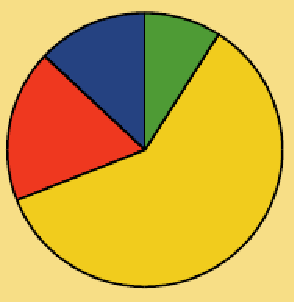
\includegraphics[width=6cm]{53_diag.pdf}
\hspace{2cm}
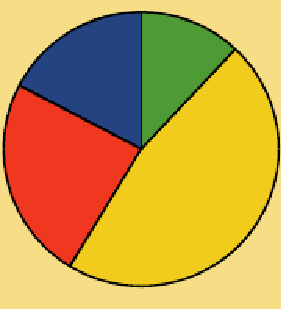
\includegraphics[width=6cm]{54_diag.pdf}
            \end{center}
            

    \end{enumerate}
    
\end{mental}

\end{MentalActivity}<++>

%+++++++++++++++++++++++++++++++++++++++++++++++++++++++++++++++++++++++++++++++++++++++++++++++++++++++++++++++++++++++++++ 
\section{Mental 5B}
%+++++++++++++++++++++++++++++++++++++++++++++++++++++++++++++++++++++++++++++++++++++++++++++++++++++++++++++++++++++++++++
\setcounter{numactivmentale}{0}

% Pour 5B, 20 février 2015
\begin{MentalActivity}  
% This is part of Un soupçon de mathématique sans être agressif pour autant
% Copyright (c) 2015
%   Laurent Claessens
% See the file fdl-1.3.txt for copying conditions.

\begin{mental}
Quelles sont les coordonnées des points \( A\), \( B\), \( C\) et \( D\) ?
\begin{center}
   \input{Fig_KBOKooTCswpl.pstricks}
\end{center}
\end{mental}





% This is part of Un soupçon de mathématique sans être agressif pour autant
% Copyright (c) 2015
%   Laurent Claessens
% See the file fdl-1.3.txt for copying conditions.

    \begin{mental}
        Compléter les pointillés :
        \begin{enumerate}
            \item
                \( 7a+3a=\ldots\times a\)
            \item
                \( 7\times 54+\ldots\times 54=540\)
        \end{enumerate}
    \end{mental}

% This is part of Un soupçon de mathématique sans être agressif pour autant
% Copyright (c) 2015
%   Laurent Claessens
% See the file fdl-1.3.txt for copying conditions.

\begin{mental}
    Développer et réduire :
    \begin{enumerate}
        \item
            \begin{equation}
                5\times (12-x)
            \end{equation}
        \item
            \begin{equation}
                5\times (12-x)+x
            \end{equation}
    \end{enumerate}
\end{mental}

\end{MentalActivity}

% Pour 5B 20 mars 2015
\begin{MentalActivity}  
% This is part of Un soupçon de mathématique sans être agressif pour autant
% Copyright (c) 2015
%   Laurent Claessens
% See the file fdl-1.3.txt for copying conditions.

    \begin{mental}
        Est-ce que les points \( A\), \( O\) et \( C\) sont alignés ?
\begin{center}
    \large
   \input{Fig_FBTCooBKTryQ.pstricks}
\end{center}
    \end{mental}
   % somme des angles plat fait 180
% This is part of Un soupçon de mathématique sans être agressif pour autant
% Copyright (c) 2015
%   Laurent Claessens
% See the file fdl-1.3.txt for copying conditions.

    \begin{mental}
        Les points \( A'\), \( B'\) et \( C'\) sont symétriques de \( A\), \( B\) et \( C\) par rapport au point \( O\). 
        \begin{center}
            \large
            \input{Fig_ZZPQooStuRcw.pstricks}
        \end{center}
        Quelle est l'aire du triangle \( A'B'C'\) ?
    \end{mental}
     % Symétrie centrale
% This is part of Un soupçon de mathématique sans être agressif pour autant
% Copyright (c) 2015
%   Laurent Claessens
% See the file fdl-1.3.txt for copying conditions.

\begin{mental}
    Calculer :
    \begin{enumerate}
        \item
            \( 7-5\)
        \item
            \( 5-7\)
        \item
            \( \frac{ 1 }{2}-1\)
    \end{enumerate}

    \vspace{2cm}

\begin{center}
   \input{Fig_FSQMooFDOrkR.pstricks}
\end{center}

\end{mental}

\end{MentalActivity}  

% Déjà fait
\begin{MentalActivity}
% This is part of Un soupçon de mathématique sans être agressif pour autant
% Copyright (c) 2015
%   Laurent Claessens
% See the file fdl-1.3.txt for copying conditions.

\begin{mental}
Est-ce que les deux droites sont parallèles ?
\begin{center}
    \large
   \input{Fig_MWIPooDUJRIo.pstricks}
\end{center}
\end{mental}

% This is part of Un soupçon de mathématique sans être agressif pour autant
% Copyright (c) 2015
%   Laurent Claessens
% See the file fdl-1.3.txt for copying conditions.

\begin{mental}
    Développer :
    \begin{enumerate}
        \item
            \( 5\times (x+3)\)
        \item
            \( 5\times (2x+3)\)
    \end{enumerate}
\end{mental}

% This is part of Un soupçon de mathématique sans être agressif pour autant
% Copyright (c) 2015
%   Laurent Claessens
% See the file fdl-1.3.txt for copying conditions.

\begin{mental}
    Si \SI{200}{\gram} de chocolat coûtent un euro, combien coûtent \SI{1.5}{\kilo\gram} ?
\end{mental}

\end{MentalActivity}

% Pour le 10 avril
\begin{MentalActivity}
% This is part of Un soupçon de mathématique sans être agressif pour autant
% Copyright (c) 2015
%   Laurent Claessens
% See the file fdl-1.3.txt for copying conditions.

\begin{mental}
    Quelle distance parcout-t-on en marchant à vitesse constante pendant \( 90\) minutes à \SI{5}{\kilo\meter\per\hour} ?
\end{mental}

% This is part of Un soupçon de mathématique sans être agressif pour autant
% Copyright (c) 2015
%   Laurent Claessens
% See the file fdl-1.3.txt for copying conditions.

\begin{mental}
    
    \begin{center}
    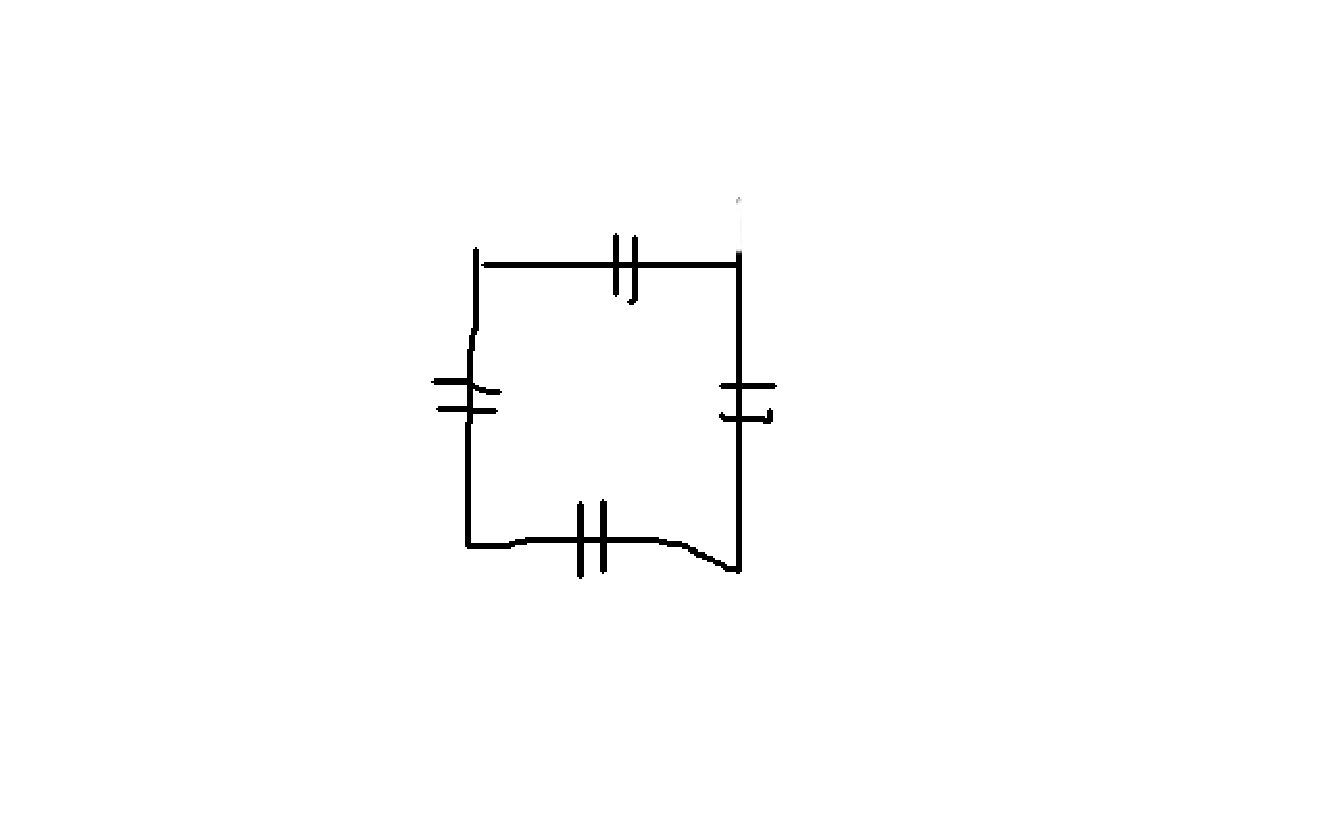
\includegraphics[width=10cm]{faux_loz_ment.pdf}
    \end{center}

Parallélogramme, losange, rectangle ou carré ?

\end{mental}

% This is part of Un soupçon de mathématique sans être agressif pour autant
% Copyright (c) 2015
%   Laurent Claessens
% See the file fdl-1.3.txt for copying conditions.

\begin{mental}
    Calculer :
    \begin{enumerate}
        \item
            \( 5-3\)
        \item
            \( 3-5\)
        \item
            \( -3+5\)
    \end{enumerate}
\end{mental}

\end{MentalActivity}

% Pour le 15 mai
\begin{MentalActivity}
% This is part of Un soupçon de mathématique sans être agressif pour autant
% Copyright (c) 2015
%   Laurent Claessens
% See the file fdl-1.3.txt for copying conditions.

\begin{mental}

Parmi les affirmation suivantes, lesquelles sont correctes ?

\begin{center}
    \input{Fig_UVWMooNNnbbG.pstricks}
\end{center}

\begin{enumerate}
    \item
        Lequel des deux périmètres est le plus grand ?
    \item
        Laquelle des deux aires est la plus grande ?
\end{enumerate}

\end{mental}

% This is part of Un soupçon de mathématique sans être agressif pour autant
% Copyright (c) 2015
%   Laurent Claessens
% See the file fdl-1.3.txt for copying conditions.

\begin{mental}
    Vrai ou faux ?
    \begin{enumerate}
        \item
            Si \( x> 10\) alors \( x+5>14\)
        \item
            Si \( x\) est un nombre quelconque alors \( x+3\) est plus grand que \( 2\).
    \end{enumerate}
\end{mental}

% This is part of Un soupçon de mathématique sans être agressif pour autant
% Copyright (c) 2015
%   Laurent Claessens
% See the file fdl-1.3.txt for copying conditions.

\begin{mental}


    \begin{center}
        \input{Fig_BXFFooNyvPYY.pstricks}
    \end{center}

    Aire de \( AKC=\ldots\)
\end{mental}

\end{MentalActivity}

% Pour le 22 mai
\begin{MentalActivity}
% This is part of Un soupçon de mathématique sans être agressif pour autant
% Copyright (c) 2015
%   Laurent Claessens
% See the file fdl-1.3.txt for copying conditions.

\begin{mental}
    \begin{enumerate}
        \item
            Combien d'euros et de centimes dans \( 1.5\)€ ?
        \item
            Combien d'heures et de minutes dans \SI{1.5}{\hour} ?
        \item
            Combien de kilos et de grammes dans \SI{1.5}{\kilo\gram} ?
    \end{enumerate}
\end{mental}

% This is part of Un soupçon de mathématique sans être agressif pour autant
% Copyright (c) 2015
%   Laurent Claessens
% See the file fdl-1.3.txt for copying conditions.


\begin{mental}
    
Sur ce dessin, \( (BD)\) est perpendiculaire à \( (BC)\).


\begin{center}
\input{Fig_HRIVooBXxZES.pstricks}
\end{center}

\end{mental}


% This is part of Un soupçon de mathématique sans être agressif pour autant
% Copyright (c) 2015
%   Laurent Claessens
% See the file fdl-1.3.txt for copying conditions.

\begin{mental}
    Laquelle de ces deux égalités est correcte si \( x=-100\) ?

    \begin{enumerate}
        \item
    $100-x=0$
\item
    $x+100=0$
    \end{enumerate}
\end{mental}


\end{MentalActivity}

% Pour le 29 mai
\begin{MentalActivity}
% This is part of Un soupçon de mathématique sans être agressif pour autant
% Copyright (c) 2015
%   Laurent Claessens
% See the file fdl-1.3.txt for copying conditions.

\begin{mental}
    Exprimer sous forme de fractions :
        \begin{enumerate}
            \item
                \( 3\times \dfrac{ 7 }{ 5 }\)
            \item
                \( 5\times \dfrac{ 9 }{ 15 }\)
        \end{enumerate}
\end{mental}

% This is part of Un soupçon de mathématique sans être agressif pour autant
% Copyright (c) 2015
%   Laurent Claessens
% See the file fdl-1.3.txt for copying conditions.

\begin{mental}
    Quel est le plus grand ?
    \begin{enumerate}
        \item
            \SI{1}{\hour}\SI{50}{\minute} ou \SI{150}{\minute} ?
        \item
            \SI{15}{€} ou \SI{150}{centimes} ?
        \item
            \SI{1}{\meter\squared} ou \SI{100}{\centi\meter\squared} ?
    \end{enumerate}
\end{mental}

% This is part of Un soupçon de mathématique sans être agressif pour autant
% Copyright (c) 2015
%   Laurent Claessens
% See the file fdl-1.3.txt for copying conditions.

\begin{mental}

    \( ABCD\) est un parallélogramme.

\begin{center}                                                                                                                    
   \input{Fig_HUGKooTkDsOg.pstricks}                                                                                    
\end{center}    

\end{mental}


\end{MentalActivity}

% Pour le 12 juin
\begin{MentalActivity}
% This is part of Un soupçon de mathématique sans être agressif pour autant
% Copyright (c) 2015
%   Laurent Claessens
% See the file fdl-1.3.txt for copying conditions.

\begin{mental}
    
Voici les éphémérides d'une éclipse\cite{PMUPooZAPegi}.
    \begin{center}
    \begin{tabular}[]{|c|c|}
        \hline
        Entrée dans l'ombre&6h58\\
        \hline
        Commencement de la totalité de l'éclipse&8h06\\
        \hline
        Maximum de l'éclipse&8h45\\
        \hline
        Fin de la totalité de l'éclipse&9h24\\
        \hline
        Sortie de l'ombre de la Terre&10h33\\
        \hline
    \end{tabular}
    \end{center}
    Pendant combien de temps l'éclipse est-elle totale ?

\end{mental}

% This is part of Un soupçon de mathématique sans être agressif pour autant
% Copyright (c) 2015
%   Laurent Claessens
% See the file fdl-1.3.txt for copying conditions.


\begin{mental}

\begin{center}
    \large
   \input{Fig_KYVAooVmGYhS.pstricks}
\end{center}

    \( \hat K=\ldots\)
\end{mental}

% This is part of Un soupçon de mathématique sans être agressif pour autant
% Copyright (c) 2015
%   Laurent Claessens
% See the file fdl-1.3.txt for copying conditions.

\begin{mental}
Quel est l'intrus ?
\begin{multicols}{2}
\begin{enumerate}
    \item
        \( 25\%\)
    \item
        \( \dfrac{1}{ 25 }\)
    \item
        \( 0.25\)
    \item
        \( \dfrac{ 25 }{ 100 }\)
    \item
        \( \dfrac{ 50 }{ 200 }\)
\end{enumerate}
\end{multicols}
\end{mental}

\end{MentalActivity}

% Pour le 16 juin
\begin{MentalActivity}
% This is part of Un soupçon de mathématique sans être agressif pour autant
% Copyright (c) 2015
%   Laurent Claessens
% See the file fdl-1.3.txt for copying conditions.

\begin{mental}
    
    Quelle est la longueur totale des arrêtes ?

\begin{center}
    \input{Fig_GJMFooFKVCyK.pstricks}
\end{center}

\end{mental}
 % Fait avec 5A
% This is part of Un soupçon de mathématique sans être agressif pour autant
% Copyright (c) 2015
%   Laurent Claessens
% See the file fdl-1.3.txt for copying conditions.

\begin{mental}
    Dire \( x=4\) est solution de l'équation
    \begin{equation}
        2x+7=15
    \end{equation}
\end{mental}
<++>
  %équation
% This is part of Un soupçon de mathématique sans être agressif pour autant
% Copyright (c) 2015
%   Laurent Claessens
% See the file fdl-1.3.txt for copying conditions.

\begin{mental}
    \( ABCD\) est un carré, et \( \widehat{AEL}=\SI{80}{\degree}\).

    \begin{center}
\input{Fig_LIWGooNsyZBz.pstricks}
    \end{center}

    \( \widehat{AKD}=\,?\)
\end{mental}

\end{MentalActivity}

%+++++++++++++++++++++++++++++++++++++++++++++++++++++++++++++++++++++++++++++++++++++++++++++++++++++++++++++++++++++++++++ 
\section{En réserve pour plus tard}
%+++++++++++++++++++++++++++++++++++++++++++++++++++++++++++++++++++++++++++++++++++++++++++++++++++++++++++++++++++++++++++

\setcounter{numactivmentale}{999}

\begin{MentalActivity}
% This is part of Un soupçon de mathématique sans être agressif pour autant
% Copyright (c) 2015
%   Laurent Claessens
% See the file fdl-1.3.txt for copying conditions.

\begin{mental}
    
\begin{center}
    \input{Fig_SXKLooPzFTnQ.pstricks}
\end{center}
\end{mental}

% This is part of Un soupçon de mathématique sans être agressif pour autant
% Copyright (c) 2015
%   Laurent Claessens
% See the file fdl-1.3.txt for copying conditions.

\begin{mental}
    
    Quelle durée s'écoule entre 15h57 et 17h08 ?
    \begin{enumerate}
        \item
            1h11
        \item
            2h11
        \item
            1h51
    \end{enumerate}

\end{mental}

% This is part of Un soupçon de mathématique sans être agressif pour autant
% Copyright (c) 2015
%   Laurent Claessens
% See the file fdl-1.3.txt for copying conditions.

\begin{mental}
    
    Sur cette figure\cite{NRHooXFvgpp5}, les traits en pointillés mesurent $\SI{2a}{\centi\meter}$ et les traits pleins mesurent \( \SI{a}{\centi\meter}\).

\begin{center}
    \input{Fig_CXDBooJMfhRr.pstricks}
\end{center}

\begin{enumerate}
    \item
        
Exprimer le périmètre en fonction de $a$.

\item

Calculer ce deux périmètres pour \( a=1.5\).
\end{enumerate}
\end{mental}




% This is part of Un soupçon de mathématique sans être agressif pour autant
% Copyright (c) 2015
%   Laurent Claessens
% See the file fdl-1.3.txt for copying conditions.

\begin{mental}
    Xavier va se coucher à \( 22h12\) et doit régler la temporisation de sa machine à laver de telle sorte qu'elle démarre à \( 5h\) du matin. Que doit-il faire ?
\end{mental}

\end{MentalActivity}

% Il faudrait un calcul mental de différence de fraction dont la réponse est zéro.
% longueur, masses, durées
% Savoir tester si une égalité comportant un ou deux nombres indéterminés est vraie lorsqu'on leur attribue des valeurs numériques.

